\documentclass[12pt]{article}

\title{Newtonian gravitation for C++ programmers}
\author{S. Halayka\footnote{sjhalayka@gmail.com}}
\date{\today\;\currenttime}

\usepackage{datetime}
\usepackage{listings}
\usepackage{cite}
\usepackage{xcolor}
\usepackage{graphicx}
\usepackage{setspace}
\usepackage{amsmath}
\usepackage{url}
\usepackage[margin=1.0in]{geometry}
\usepackage{listings}


\usepackage{xcolor}
\lstset { %
    language=C++,
    backgroundcolor=\color{black!5}, % set backgroundcolor
    basicstyle=\footnotesize,% basic font setting
    showstringspaces=false,
}


%\doublespace

%\usepackage[]{lineno}
%\linenumbers


\begin{document}



 
\maketitle

\begin{abstract}
...
\end{abstract}



\section{Typedefs}

\begin{lstlisting}
typedef long double real_type;
\end{lstlisting}

or

\begin{lstlisting}
#include <boost/multiprecision/cpp_bin_float.hpp>
using namespace boost::multiprecision;

typedef number<
	backends::cpp_bin_float<
		237, 
		backends::digit_base_2, 
		void, 
		std::int32_t, 
		-262142, 
		262143>, 
	et_off> cpp_bin_float_oct;

typedef cpp_bin_float_oct real_type;
\end{lstlisting}





\section{Constants}

\begin{lstlisting}
const real type dt = 10000; // 2.77777 hours

const real_type pi = 4.0 * atan(1.0);

const real_type G = 6.67430e-11;
const real_type c = 299792458;
const real_type c2 = c * c;
const real_type c3 = c * c * c;
const real_type c4 = c * c * c * c;
const real_type h = 6.62607015e-34;
const real_type hbar = h / (2.0 * pi);
\end{lstlisting}






\section{Brute force: integer field line count}

Where $r$ is the receiver radius, $R$ is the distance from the centre of the emitter, $\beta$ is the get intersecting line count function, and $n$ is the field line count, the gradient is:
\begin{equation}
\alpha = \frac{\beta(R + \epsilon) - \beta(R)}{\epsilon}.
\end{equation}
The gradient strength is:
\begin{equation}
g = \frac{-\alpha}{r^2}.
\end{equation}

\begin{lstlisting}
long long unsigned int get_intersecting_line_count(
	const vector<vector_3>& unit_vectors,
	const vector_3& sphere_location,
	const real_type sphere_radius)
{
	long long unsigned int count = 0;

	vector_3 cross_section_edge_dir(sphere_location.x, sphere_radius, 0);
	cross_section_edge_dir.normalize();

	vector_3 receiver_dir(sphere_location.x, 0, 0);
	receiver_dir.normalize();

	const real_type min_dot = cross_section_edge_dir.dot(receiver_dir);

	for (size_t i = 0; i < unit_vectors.size(); i++)
		if (unit_vectors[i].dot(receiver_dir) >= min_dot)
			count++;

	return count;
}
\end{lstlisting}

\begin{lstlisting}
int main(int argc, char** argv)
{
	// Field line count
	const size_t n = 1000000000;

	cout << "Allocating memory for field lines" << endl;
	vector<vector_3> unit_vectors(n);

	for (size_t i = 0; i < n; i++)
	{
		unit_vectors[i] = RandomUnitVector();

		static const size_t output_mod = 10000;

		if (i % output_mod == 0)
			cout << "Getting pseudorandom locations: " 
			<< static_cast<float>(i) / n << endl;
	}

	string filename = "newton.txt";
	ofstream out_file(filename.c_str());
	out_file << setprecision(30);

	const real_type start_distance = 10.0;
	const real_type end_distance = 100.0;
	const size_t distance_res = 1000;

	const real_type distance_step_size = 
		(end_distance - start_distance) 
		/ (distance_res - 1);

	for (size_t step_index = 0; step_index < distance_res; step_index++)
	{
		const real_type r = 
			start_distance + 
			step_index * distance_step_size;

		const vector_3 receiver_pos(r, 0, 0);
		const real_type receiver_radius = 1.0;

		const real_type epsilon = 1.0;

		vector_3 receiver_pos_plus = receiver_pos;
		receiver_pos_plus.x += epsilon;

		const long long signed int collision_count_plus = 
			get_intersecting_line_count(
				unit_vectors, 
				receiver_pos_plus, 
				receiver_radius);
		
		const long long signed int collision_count = 
			get_intersecting_line_count(
				unit_vectors, 
				receiver_pos, 
				receiver_radius);
		
		const real_type gradient = 
			static_cast<real_type>
			(collision_count_plus - collision_count) 
			/ epsilon;
		
		const real_type gradient_strength = 
			-gradient 
			/ (receiver_radius * receiver_radius);

		cout << "r: " << r << " gradient strength: " 
		<< gradient_strength << endl;

		out_file << r << " " << gradient_strength << endl;
	}

	out_file.close();

	return 0;
}
\end{lstlisting}

While this method works, it is both memory and processor intensive.
Thus, this method is meant to be a stepping stone for the next section.

\begin{figure} 
\centering
  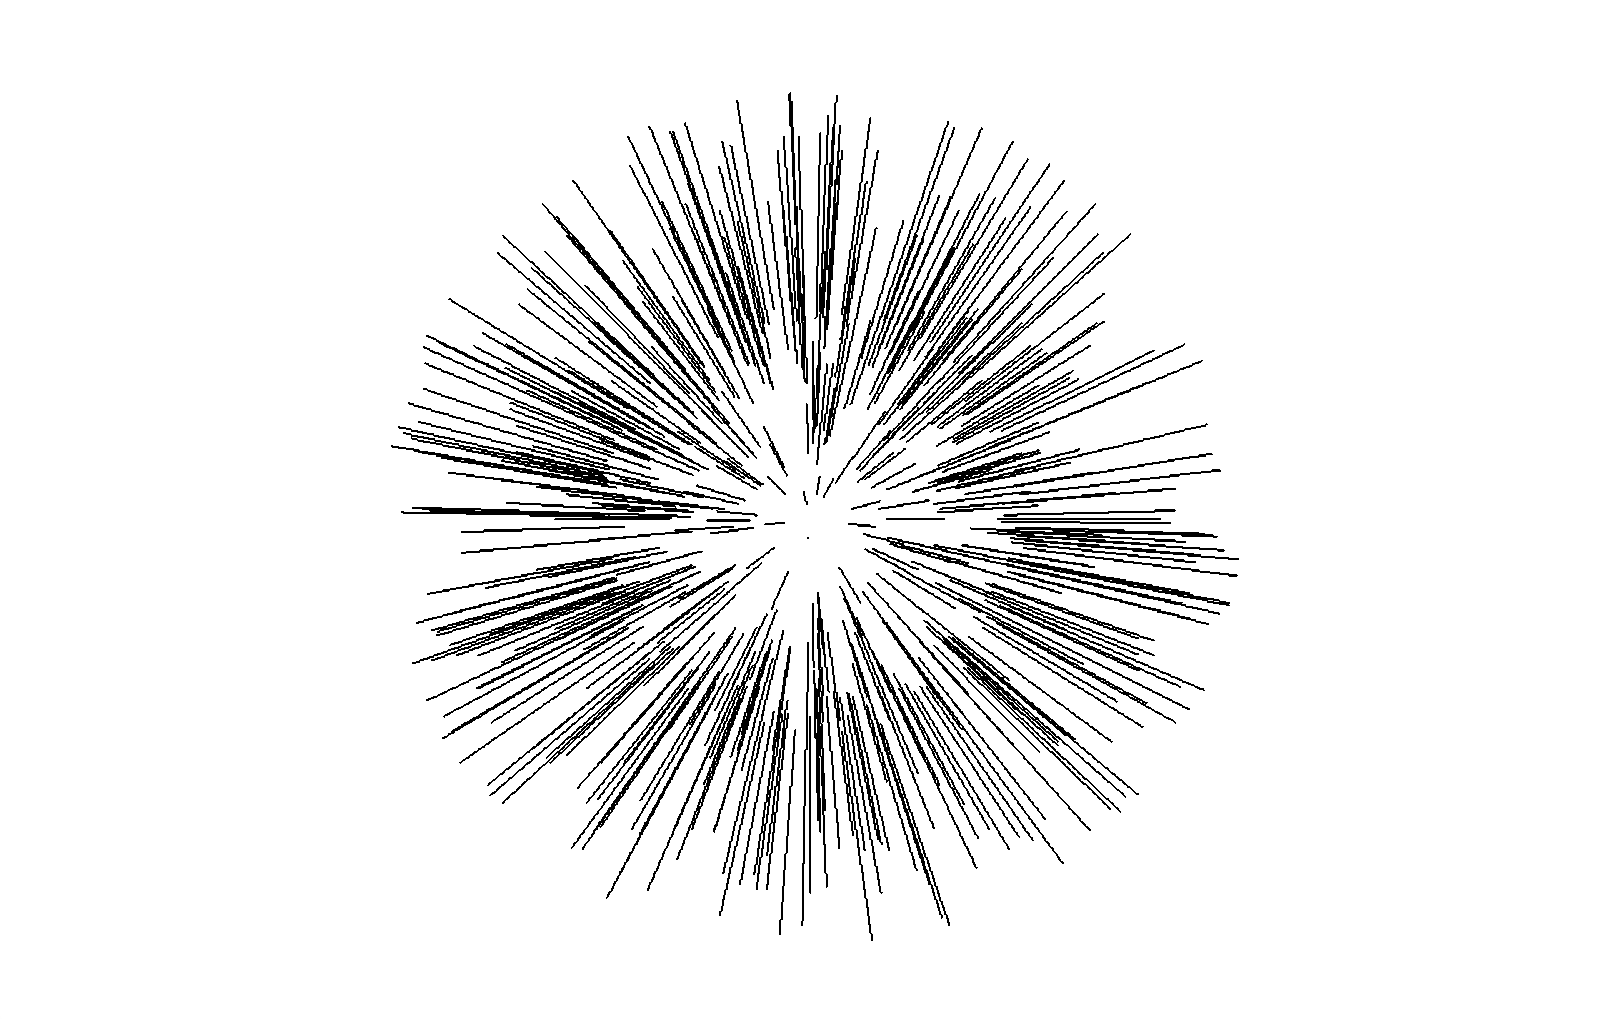
\includegraphics[width = 5 in]{3.png}
  \caption{
Example of an isotropic emitter.
The emitter is spherical.
The field line starting locations are placed pseudorandomly on a 2-sphere, and the normals (e.g. field line directions) are calculated using the same sphere.
}
\end{figure}

\section{Heuristic: real field line count}

Where $r$ is the receiver radius, $R$ is the distance from the centre of the emitter, $\beta$ is the get intersecting line count function, and $n$ is the field line count, the gradient is:
\begin{equation}
\alpha = \frac{\beta(R + \epsilon) - \beta(R)}{\epsilon}.
\end{equation}

Here we assume that the maximum number of field lines is given by the holographic principle:
\begin{equation}
n = \frac{A c^3}{ 4 G \hbar \log 2}.
\end{equation}

The gradient strengths are:
\begin{equation}
g = \frac{-\alpha}{r^2} \approx \frac{n}{2 R^3},
\end{equation}
\begin{equation}
g_N = \frac{g R c \hbar \log 2}{2 \pi M} = \frac{n c \hbar \log 2}{4 \pi M R^2} = \frac{A c^4}{16 \pi G M R^2} = \frac{G M}{R^2}.
\end{equation}



\begin{lstlisting}
real_type get_intersecting_line_count(
	const real_type n,
	const vector_3& sphere_location,
	const real_type sphere_radius)
{
	const real_type big_area = 
		4 * pi * sphere_location.x * sphere_location.x;

	const real_type small_area = 
		pi * sphere_radius * sphere_radius;
	
	const real_type ratio = 
		small_area / big_area;
	
	return n * ratio;
}
\end{lstlisting}



\begin{lstlisting}
int main(int argc, char** argv)
{
	const real_type emitter_radius = 1.0;
	
	const real_type emitter_area = 
		4.0 * pi * emitter_radius * emitter_radius;

	// Field line count
	// re: holographic principle:
	const real_type n = 
		(c3 * emitter_area) 
		/ (log(2.0) * 4.0 * G * hbar);
	
	const real_type emitter_mass = c2 * emitter_radius / (2.0 * G);

	// 1.73502e+70 is the 't Hooft-Susskind constant:
	// the number of field lines for a black hole of
	// unit Schwarzschild radius
	//
	//const real_type G_ = 
	//	(c3 * pi) 
	//	/ (log(2.0) * hbar * 1.73502e+70);

	const string filename = "newton.txt";
	ofstream out_file(filename.c_str());
	out_file << setprecision(30);

	const real_type start_distance = 10.0;
	const real_type end_distance = 100.0;
	const size_t distance_res = 1000;

	const real_type distance_step_size =
		(end_distance - start_distance)
		/ (distance_res - 1);

	for (size_t step_index = 0; step_index < distance_res; step_index++)
	{
		const real_type r =
			start_distance + step_index * distance_step_size;

		const vector_3 receiver_pos(r, 0, 0);
		const real_type receiver_radius = 1.0;

		const real_type epsilon = 1.0;

		vector_3 receiver_pos_plus = receiver_pos;
		receiver_pos_plus.x += epsilon;

		// https://en.wikipedia.org/wiki/Directional_derivative
		const real_type collision_count_plus =
			get_intersecting_line_count(
				n,
				receiver_pos_plus,
				receiver_radius);

		const real_type collision_count =
			get_intersecting_line_count(
				n,
				receiver_pos,
				receiver_radius);

		const real_type gradient =
			(collision_count_plus - collision_count)
			/ epsilon;

		real_type gradient_strength =
			-gradient
			/ (receiver_radius * receiver_radius);

		const real_type gradient_strength_ = 
			n / (2.0 * pow(receiver_pos.x, 3.0));

		const real_type newton_strength = 
			n * c * hbar * log(2.0)
			/ 
			(pow(receiver_pos.x, 2.0) 
				* emitter_mass * 4.0 * pi);

		const real_type newton_strength_ =
			c4 * emitter_area
			/ (16.0 * pi * G 
				* pow(receiver_pos.x, 2.0) * emitter_mass);

		const real_type newton_strength__ =
			G * emitter_mass / pow(receiver_pos.x, 2.0);

		const real_type newton_strength___ =
			gradient_strength_ * receiver_pos.x 
			* c * hbar * log(2)
			/ (2 * pi * emitter_mass);

		//cout << newton_strength___ / newton_strength << endl;

		cout << "r: " << r << " gradient strength: "
			<< gradient_strength << endl;

		out_file << r << " " << gradient_strength << endl;
	}

	out_file.close();

	return 0;
}
\end{lstlisting}

This method is faster and less memory intensive when compared to the integer field count method.
This method is meant to be a stepping stone for the next section.




\section{Application: modeling Mercury's orbit using numerical integration}

The initial conditions are:
\begin{lstlisting}
vector_3 Mercury_pos(0, 69817079000.0, 0);
vector_3 Mercury_vel(-38860, 0, 0);
\end{lstlisting}

The orbit code is:
\begin{lstlisting}
vector_3 Newtonian_acceleration(
	const real_type emitter_mass,
	const vector_3& pos, // Receiver pos
	const real_type G)
{
	vector_3 grav_dir = vector_3(0, 0, 0) - pos;
	const real_type distance = grav_dir.length();
	grav_dir.normalize();

	vector_3 accel = grav_dir * G * emitter_mass / pow(distance, 2.0);

	return accel;
}
\end{lstlisting}

Here we show the Euler integration, which is extremely simple:
\begin{lstlisting}
void proceed_Euler(
	vector_3& pos, 
	vector_3& vel, 
	const real_type G, 
	const real_type dt)
{
	vector_3 accel = 
		Newtonian_acceleration(
			emitter_mass, 
			pos, 
			G);

	vel += accel * dt;
	pos += vel * dt;
}

\end{lstlisting}

And so the passage of time is computed as:
\begin{lstlisting}
void idle_func(void)
{
	proceed_Euler(Mercury_pos, Mercury_vel, G, dt);
}
\end{lstlisting}



On the other hand, rather than using Euler integration, the order-4 symplectic integration does a better job at conserving energy, but at a speed cost:
\begin{lstlisting}
void proceed_symplectic_order_4(
	vector_3& pos, 
	vector_3& vel, 
	real_type G, 
	real_type dt)
{
	static const real_type cr2 = 
		pow(2.0, 1.0 / 3.0);

	static const real_type c[4] =
	{
		1.0 / (2.0 * (2.0 - cr2)),
		(1.0 - cr2) / (2.0 * (2.0 - cr2)),
		(1.0 - cr2) / (2.0 * (2.0 - cr2)),
		1.0 / (2.0 * (2.0 - cr2))
	};

	static const real_type d[4] =
	{
		1.0 / (2.0 - cr2),
		-cr2 / (2.0 - cr2),
		1.0 / (2.0 - cr2),
		0.0
	};

	pos += vel * c[0] * dt;
	vel += Newtonian_acceleration(
			emitter_mass, 
			pos, 
			G) * d[0] * dt;

	pos += vel * c[1] * dt;
	vel += Newtonian_acceleration(
			emitter_mass, 
			pos, 
			G) * d[1] * dt;

	pos += vel * c[2] * dt;
	vel += Newtonian_acceleration(
			emitter_mass, 
			pos, 
			G) * d[2] * dt;

	pos += vel * c[3] * dt;
	// last element d[3] is always 0
}
\end{lstlisting}








\section{Final code}

A final code, which models the orbit of Mercury, is at:

\url{https://github.com/sjhalayka/mercury_orbit_glut}

\begin{figure} 
\centering
  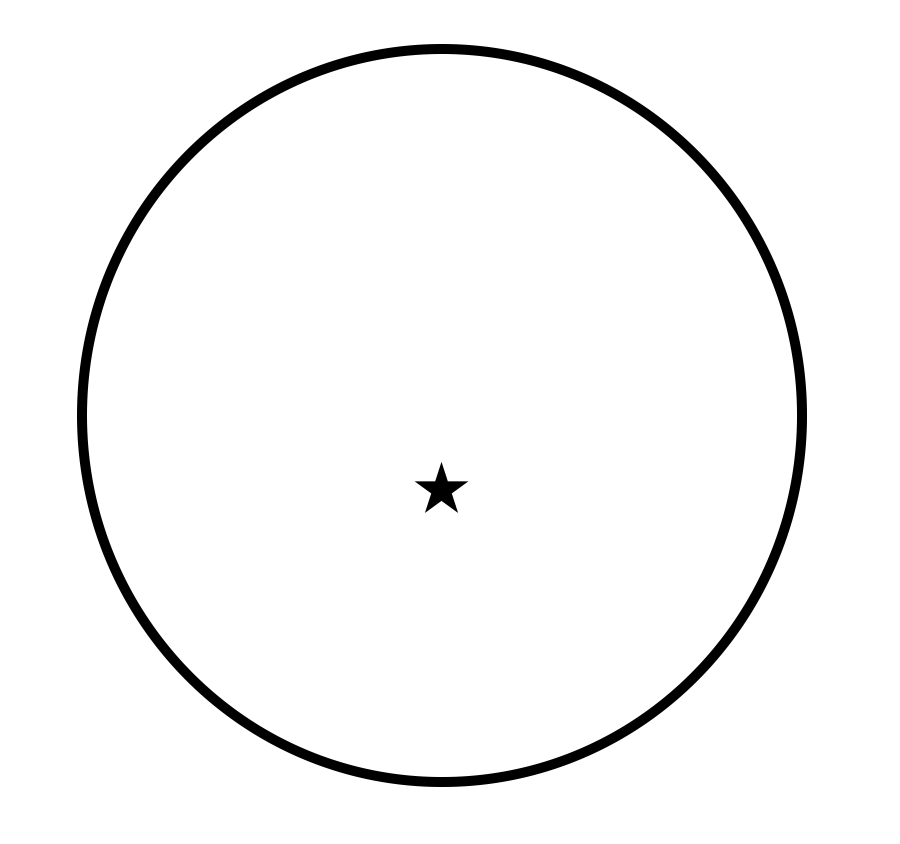
\includegraphics[width = 5 in]{mercury.png}
  \caption{
Mercury in orbit around the Sun.
}
\end{figure}




%\begin{thebibliography}{9}




%\end{thebibliography}






\end{document}









